\documentclass[conference]{IEEEtran}
\IEEEoverridecommandlockouts
% The preceding line is only needed to identify funding in the first footnote. If that is unneeded, please comment it out.
\usepackage{cite}
\usepackage{amsmath,amssymb,amsfonts}
\usepackage{graphicx}
\usepackage{textcomp}
\usepackage{enumitem}
\usepackage{xcolor}
\usepackage{times}
\usepackage[binary-units=true]{siunitx}
\usepackage{latexsym}
\usepackage{hyperref}
\hypersetup{colorlinks=true,linkcolor=black,citecolor=blue,filecolor=black,urlcolor=blue}
\usepackage{algpseudocode}
\usepackage{algorithm}
\usepackage{caption}
\usepackage{subcaption}

%\setlength{\textfloatsep}{7pt}

\newcommand{\TG}[1]{\color{cyan}From Tristan: #1 \color{black}}
\newcommand{\MD}[1]{\color{magenta}From Mathieu: #1 \color{black}}
\newcommand{\VHS}[1]{\color{green}From Valerie: #1 \color{black}}

\begin{document}

\title{Performance comparison of Dask and Apache Spark on HPC systems}

\author{Mathieu Dugr\'e, Val\'erie Hayot-Sasson, Tristan Glatard\\
	Department of Computer Science and Software Engineering\\
	Concordia University, Montr\'eal, Qu\'ebec, Canada\\
	\{mathieu.dugre, valerie.hayot-sasson, tristan.glatard\}@concordia.ca
	\vspace*{0.8cm} % to avoid weird spacing of 1st page by Latex.
}

\maketitle

\begin{abstract}
	% TODO
\end{abstract}

\begin{IEEEkeywords}
	Performance, Big Data, Dask, Spark, Neuroimaging, HPC
\end{IEEEkeywords}

\section{Introduction}
The rise in data sharing coupled with improved data collection technologies leads neuroimaging into the Big Data era\cite{ALFAROALMAGRO:18, van2014human, ConpPortal}.
While standard neuroimaging workflow engines, such as Nipype\cite{Nipype:11}, are well rounded to process standard compute-intensive pipelines,
they lack Big Data strategies (i.e., in-memory computing, data locality, and lazy-evaluation) to improve the performance of increasingly prevalent data-intensive pipelines.
A previous study\cite{hayot2019performance} noted the importance of in-memory computing and data locality to improve the performance of data-intensive pipelines.
In this work, we study how performance benchmarks generalize across Big Data engines in an HPC environment.
In particular, we study in-depth the performance difference between Dask\cite{Dask:15} and Apache Spark\cite{Spark:16} for their suitability to process neuroimaging pipelines.
Our objective is to assess whether Spark or Dask has substantial performance benefits in processing data-intensive HPC clusters pipelines.

Spark and Dask both provide in-memory computing, data locality, and lazy-evaluation, typical for Big Data engines.
The scheduler for both engines operates dynamically, which benefits applications with runtime unknown ahead of time\cite{Dask:15}.
They also provide rich high-level API and support a variety of schedulers and deployment environments, such as Mesos\cite{hindman2011mesos}, YARN\cite{vavilapalli2013apache}, Kubernetes, and HPC clusters.
Although sharing similarities, these engines have differences.

First and foremost, Spark is written in Scala while Dask is in Python.
The popularity of Python in the scientific community arguably gives an edge to Dask due to the serialization cost between Python and Scala.
However, if not careful, the Python Global Interpreter Lock (GIL) can significantly reduce the parallelism of an application in some cases.
The difference in programming languages also provides different benefits.
On the one hand, as part of the Scipy ecosystem, Dask provides almost transparent integration with APIs such as Numpy arrays, Pandas dataframe, or RAPIDS GPU accelerated code framework.
On the other hand, Spark's Java, Scala, R, and Python APIs efficiently parallelize pipelines with minimal performance loss, thanks to the Java Virtual Machine. \TG{you could add a few words to explain why the JVM is useful for parallelization ("thanks to the JVM that ...")}
Our study is restrained to performance, although we recognize that other factors affect the choice of an engine in practice.

While laptops or workstations can be sufficient for some applications, data-intensive neuroimaging pipelines often require large infrastructures.
This paper focuses on the performance of Big Data engines in HPCs environments.
We installed the Slurm scheduler and Lustre file system~\cite{braam2019lustre} on a dedicated cluster to mimic a typical HPC system.
Lustre is a powerful and scalable file system for HPC environments offering parallel file accesses.

In a previous study\cite{8943502} we found that there was no significant performance difference between Apache Spark and Dask for data-intensive applications.
However, using a network file system (NFS) led to an I/O bottleneck limiting the performance of the applications.
Another study \cite{8588652} also reported network and I/O bottlenecks when concurrency increased.
This same study found that the startup overhead time for Spark was more prominent than for Dask.
On the contrary, the work in~\cite{Mehta:17} claims that the startup overhead is more significant for Dask than for Spark.
This contradiction suggests that the startup overhead might vary depending on cluster configuration.
The latter study processed a \SI{100}{\giga\byte} dataset using a neuroimaging pipeline and found Dask to be up to 14\% faster than Spark due to ``more efficient pipelining" and serialization time to Python.
On the contrary, the work in \cite{10.1145/3225058.3225128} shows that with large datasets, Spark provides better speedup than Dask.
However, that study used the Dask Bag API, which has performance limitations compared to other Dask APIs.

The above studies compared the performance of the engine at a high level.
In comparison, our study provides a detailed analysis of the performance differences and similarities between Dask and Spark for data-intensive applications.

The following section introduces the Lustre file system and the Big Data engines.
Next, we present the design of our benchmarking experiments.
We consider two types of data-intensive neuroimaging pipelines: high-resolution imaging and functional MRI studies for a cohort of subjects.
The pipelines we chose involve different compute and I/O patterns, e.g., map-reduce or map-only, requiring partial data in memory or the whole dataset.
Further sections present our results, discussion, and conclusion.


\section{Background}
\subsection{Lustre}
The Lustre file system is a parallel file system well suited for HPC environments.
Lustre offers a POSIX-compliant interface with the file system.
Installed in some of the most powerful supercomputers, the design of Lustre allows
scaling to thousands of nodes, petabytes of storage, and hundreds of gigabits per second of I/O throughput.

At the core of Lustre are the \textit{management servers} (MGSs) and \textit{metatdata server} (MDSs) in charge of the files operations and metadata,
the \textit{object storage targets} (OSTs) to store file data, and the \textit{object sotrage server} (OSSs) to handle the OSTs.
Lustre clients make requests to the MGSs to access files on the OSTs.
To handle failures in the system, the MGSs, MDSs, and OSTs have failover capabilities.
InfiniBand, Ethernet, or a combination of both can be used to interconnect these different components.

\subsection{Dask}
Dask is a Python-based Big Data engine with growing popularity in the scientific Python ecosystem.
Dask was designed with data locality and in-memory computing in mind to mitigate the data transfer bottleneck in Big Data workflows.
Data locality, popularized by Map-Reduce \cite{dean2008mapreduce}, schedules tasks where the data reside.
In-memory computing minimizes the overhead of transferring data to disk sby keeping data in memory when possible.
Dask uses lazy evaluation to reduce unnecessary communication and computation.
The engine builds a dynamic graph before execution, allowing it to determine which task to compute.
Dask workflows can further reduce data transfer by leveraging multithreading whenever the Python GIL does not restrict it.
It achieves Fault tolerance by recording data lineage, the sequence of operations used to modify the initial data.

Dask offers five data structures:
\href{https://docs.dask.org/en/latest/array.html}{Array},
\href{https://docs.dask.org/en/latest/bag.html}{Bag},
\href{https://docs.dask.org/en/latest/dataframe.html}{DataFrame},
\href{https://docs.dask.org/en/latest/delayed.html}{Delayed},
and \href{https://docs.dask.org/en/latest/futures.html}{Futures}.
Arrays offer a clone of NumPy API for distributed processing of large arrays.
Bags are a distributed collection of Python object that offers a programming abstraction similar to \href{https://toolz.readthedocs.io/en/latest/}{PyToolz}.
Dataframes are a parallel composition of \href{https://pandas.pydata.org/}{Pandas} Dataframes used to process a large amount of tabular data.
Dask Delayed offers an API for distributing arbitrary functions that do not fit in the above frameworks.
Lastly, Dask Futures can also execute arbitrary functions; however, it launches computation immediately rather than lazily.
Dask allows users to install only required components making it lightweight.

In Dask, a scheduler decides where and when to execute tasks using the Dask graph.
API operations generate multiple fine-coarse tasks in the computation graph, allowing a more straightforward representation of complex algorithms.

The Dask engine is compatible with multiple distributed schedulers, including YARN and Mesos.
It also provides a \textit{Dask Distributed scheduler}.
We chose to use Dask Distributed scheduler to keep the environment balanced between the engines.

In the Dask Distributed scheduler, a \textit{dask-scheduler} process administrates the resource provided by \textit{dask-worker}s in the cluster.
The scheduler receives jobs from clients and assigns tasks to available workers using a global FIFO (First-In-First-Out) job scheduling policy.
However, the Dask scheduler attempts to complete immediate task dependencies using a LIFO (Last-in-First-Out) policy to reduce the memory footprint of the workers.

Dask offers multiple ways to deploy a cluster, including, but not limited to, SSH configs, Kubernetes, SLURM, PBS.
For our experiments, we used the \href{https://jobqueue.dask.org/en/latest/generated/dask_jobqueue.SLURMCluster.html}{Dask SLURM cluster} API.

\subsection{Apache Spark}
Apache Spark is a widely-used general-purpose Big Data engine.
Like Dask, it aims at reducing data transfer costs by incorporating data locality, in-memory computing, and lazy evaluation.

Spark offers three options to schedule jobs: Spark Standalone, Mesos, and YARN.
Spark Standalone is a simple built-in scheduler.
YARN is mainly used to schedule Hadoop-based workflows, while Mesos can be used for various workflows.
We limit our focus to Spark Standalone scheduler, as researchers are likely to 
execute their workflows in an HPC environment where neither YARN nor Mesos is usually available.

In the Spark Standalone scheduler, a \textit{leader} (a.k.a master) coordinates the resource provisioned by \textit{workers} in the cluster.
A \textit{driver}  process receives jobs from clients and requests workers from the leader.
Jobs are divided into stages to execute onto workers.
Each operation in a stage is represents by a high-level task in the computation graph.
Like Dask, Spark Standalone scheduler uses a LIFO policy to schedule tasks.
Spark Standalone has two execution modes: (1) the client mode, where the driver process runs in a dedicated process,
and (2) the cluster mode, where the driver runs within a worker process.
Our experiments use the client mode since cluster mode is not available in PySpark.

Spark's primary data structure is Resilient Distributed Dataset (RDD)\cite{RDD}, a fault-tolerant, parallel collection of data elements.
RDDs are the basis of the other Spark data structure: Datasets and DataFrames.
Datasets are similar to RDD but benefit additional performance by leveraging Spark SQL's optimized execution engine. 
The DataFrames are Datasets organized into named columns and are used to process tabular data. 
While the DataFrame API is available in all supported languages, Datasets are limited to Scala and Java. 

Python is a standard programming language in the scientific community, offering numerous data processing libraries.
While serialization from Python to Java, an operation required when using Spark's Python API, creates overhead, we found it minimal \cite{8943502}.
We focus on PySpark API to have a more balanced environment between the different engines and its suitability for neuroimaging.

\section{Methods}
\subsection{Infrastructure}
We used the ``slashbin" cluster at Concordia University.
The cluster has eight compute nodes, four storage nodes, one login node, and one Lustre metadata node.
Each compute node has two 16-core Intel(R) Xeon(R) Gold 6130 CPU @ 2.10GHz,
\SI{250}{\gibi\byte} of RAM, \SI{126}{\gibi\byte} of tmpfs,
% 6 $\times$ SSDs of \SI{447}{\gibi\byte} each with the XFS file system (no RAID enabled),
CentOS~8.1 and Linux kernel \textit{4.18.0-240.1.1.el8\_lustre.x86\_64}.

We configured Lustre to have 1 MGS and 4 OSS.
Each OSS has 11 OSTs (disks) of \SI{8.8}{\tebi\byte}.
The OSTs are configured to have a maximum of \SI{1000}{\mebi\byte} of dirty data written into the client page cache.
Both the MDT and OSTs are configured to a maximum of 64 concurrent RPCs in flight.
A timeout of \SI{100}{\second} is set for Lustre, and OSTs checksum are disabled.
Lustre \textit{2.14.0-1.el8} is installed on both the Lustre clients and servers.
	
Both Spark and Dask are configured to have eight worker processes, each with eight threads.
Each worker was allocated \SI{31.5}{\gibi\byte} of memory.
For Spark, the JVM heap space uses 10\% () of workers' memory, and the location of the log is set on an NFS.
The worker workspace for both engines is located on Lustre due to the limited fast storage space on the worker nodes.
Other Dask configurations are left to default.
The Spark network timeout is set to \SI{600}{\second} and the executor heartbeat to \SI{120}{\second}
A new Dask or Spark cluster was started and tore down for each experiment.
Dask \textit{2021.7.0} and Spark \textit{3.1.2} was used for our experiments.
	
\subsection{Dataset}
We used BigBrain\cite{Amunts:13}, a 3-D image of the human brain with voxel
intensities ranging from 0 to 65,535. We converted the blocks into the
NIfTI format, a popular format in neuroimaging. We left the NIfTI blocks
uncompressed, resulting in total data size of \SI{606}{\gibi\byte}. To
evaluate the effect of block size, we split the image into 1000, 2500,
and 5000 files of \SI{606}{\mebi\byte}, \SI{242.4}{\mebi\byte}, and
\SI{121.2}{\mebi\byte}, respectively.
We used the \href{https://github.com/big-data-lab-team/sam}{sam} library to split the image.
		
We also used the dataset provided by the Consortium for Reliability and
Reproducibility
(\href{http://fcon_1000.projects.nitrc.org/indi/CoRR/html/}{CoRR})
\cite{zuo2014open}, freely available on
\href{https://datasets.datalad.org/?dir=/corr/RawDataBIDS}{DataLad}.
The entire dataset is \SI{379.83}{\gibi\byte}, containing anatomical, diffusion,
and functional images of 1,654 subjects acquired in 35 sites.
We used all 3,491 anatomical images, representing \SI{26.67}{\gibi\byte} overall
(\SI{7.82}{\mebi\byte} per image on average).
		
\subsection{Applications}
In this section, we describe the applications used to benchmark Dask and Spark.
We use three simple synthetic applications to have a deep understanding of the 
underlying behavior of the applications with simple I/O pattern, namely
\textit{Increment}, \textit{Multi-Increment}, and \textit{Histogram}.
Also, two neuroimaging applications are used to study more realistic 
applications; namely \textit{Kmeans} and \textit{BIDS App Example}.
		
To have a fair comparison between the engines, the code base for the core functions of the applications is the same for both engines.
This allows us to reduce the performance difference from different implementations.
		
\subsubsection{Increment}
We adapted the increment application used in \cite{hayot2019performance}.
This synthetic application reads blocks of the BigBrain from Lustre and
simulates computation by sleeping for a specified period. To simulate
intermediate results, we repeat the sleep process for a configurable amount
of time. We prevent data caching of the blocks by incrementing their voxels
value by one after each sleep operation. Finally, we write the resulting
NIfTI image back to Lustre. This application allows us to study the engines
when their inputs are processed independently. The map-only pattern
mimics the processing of multiple independent subjects in parallel.
\begin{figure}[!ht]
	\centering
	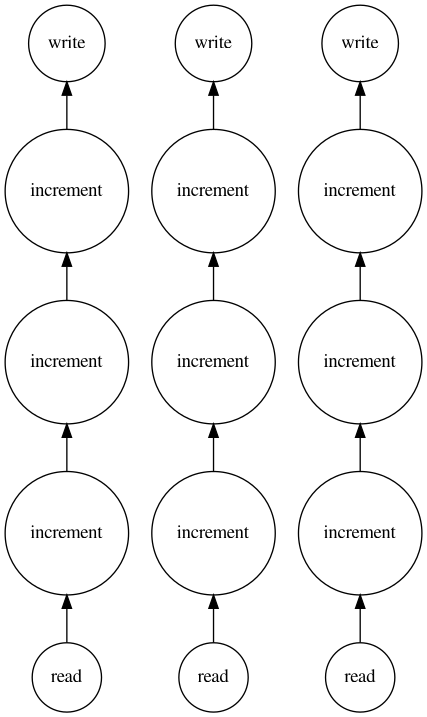
\includegraphics[height=\columnwidth,
	angle=0]{figures/increment.png}
	\caption{Task graph for Incrementation with 3 iterations and 3 BigBrain blocks.}
	\label{fig:graph-increment}
\end{figure}
			
\subsubsection{Histogram}
As our third application, we calculate the histogram of the BigBrain image. 
The application reads the BigBrain blocks from Lustre, calculates each intensity's frequency, and then writes the aggregated result back on Lustre.
This map-reduce application has a very high read overwrite ratio.
Moreover, this application requires shuffling, albeit of a limited amount of data. 
The amount of inter-worker communication is in-between the increment and multi-increment applications.
\begin{figure}[!hb]
	\centering
	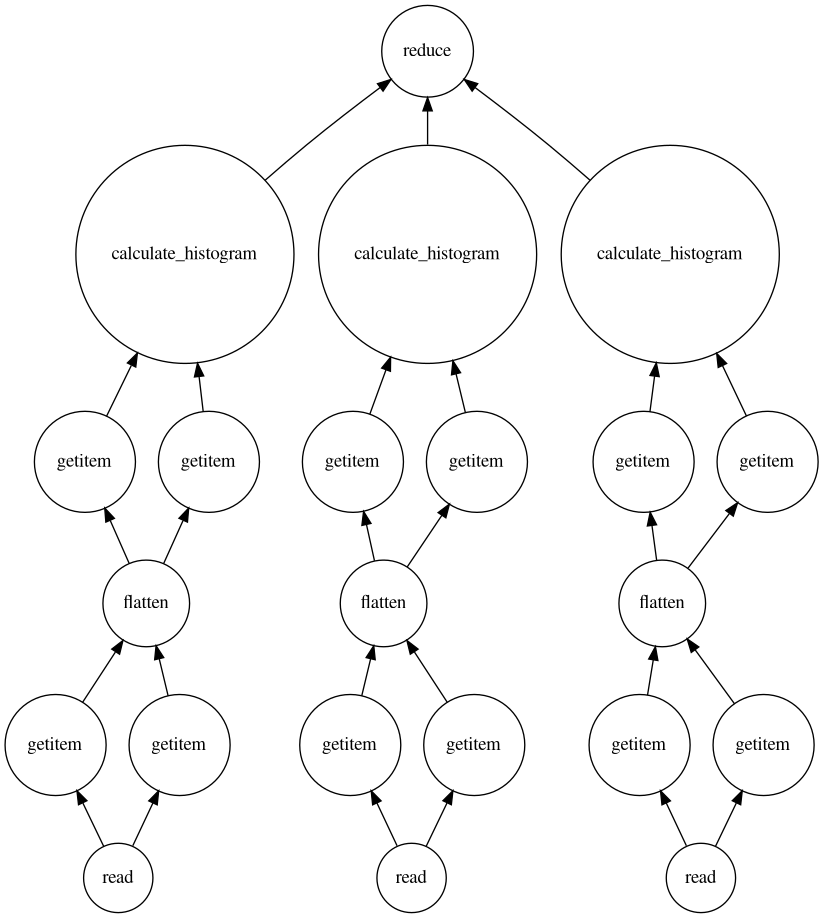
\includegraphics[height=\columnwidth,
	angle=0]{figures/histogram.png}
	\caption{Task graph for Histogram with 3 BigBrain blocks.}
	\label{fig:graph-histogram}
\end{figure}
			
\subsubsection{Kmeans}
For our fourth application, we apply Kmeans clustering to the voxel
intensities of the BigBrain image. We set the number of clusters to 3. The
application starts by reading the image blocks, combining all voxels in a
1-D array, and choosing initial centroids using the min, max, and
intermediate values. It assigns each voxel to its closest centroid and
updates each centroid with the average of its assigned voxels. It repeats
the assignment and update steps for a configurable number of iterations.
Finally, the voxels of the image blocks are classified and written back to
the file system. Updating the centroids involves substantial data
communication between the workers.
The computation to find the closest centroids for each voxels scales with the number of centroids.
It can be computed in parallel at the cost of higher memory or sequentially to reduce memory usage.
We decided to compute the nearest centroids in parallel since we use only three centroids.

\subsubsection{BIDS App example}
Our fifth application is the BIDS App example, a neuroimaging pipeline to
measure the brain volume from MRIs. For this application, we use the CoRR
dataset. The application extracts the brain volume of each participant,
then computes the average for each group of participants. Unlike the other
applications, the BIDS App example is a command-line executed in a Docker image
(bids/example on DockerHub). We converted the Docker image to a Singularity
image for use in HPC environments, \MD{Cite paper on the reason why this is
done.} using
\href{https://hub.docker.com/r/singularityware/docker2singularity/tags/}{docker2singularity}
		
\subsection{Experiments}
Table~\ref{table:parameters} shows the parameters that were varied
throughout the experiments. We varied (1) the number of workers to assess
the scalability of the engine scheduler, (2) the BigBrain
block size in Increment, Multi-Increment, and Histogram to measure the
effect of different I/O patterns and parallelization degrees, (3) the
number of iterations to evaluate the effect of the number of tasks, and (4) the
sleep delay to study the effect of task duration. It should note that
increasing the number of iterations for a given sleep delay also increases
the total compute time of an application.
		
To avoid potential external biases due to caching, background processes and,
network load, we ran the applications in randomized order and cleared the
page cache between every experiment.
Moreover, we ran each benchmark ten times.
		
For each execution, we measured the time spent in the different functions of the
application to read, process, and write data.
We calculate the overhead for each CPU thread by subtracting the total time
spent in the reading, writing, and processing functions to the makespan of the application.
Summing those results gives the total overhead for the application.
		
\begin{table*}[t]
	\renewcommand{\arraystretch}{1.5}
	\caption{Parameters for the experiments}\label{table:parameters}
	\centering
	\begin{tabular}{|l|c|c|c|c|c|}
		\hline           & Increment & Histogram & Kmeans  & BIDS App Example \\\hline
		\# of Nodes & \multicolumn{4}{c|}{2, 4, 8} \\\hline
		Dataset size [\SI{}{\gibi\byte}] &\multicolumn{2}{c|}{606} & 303 & \multicolumn{1}{c|}{26.67} \\\hline
		Number of file & \multicolumn{2}{c|}{1000, 2500, 5000} & - & \multicolumn{1}{c|}{3491} \\\hline
		\# of Iterations & 1, 5, 25  & -         & 1, 3, 9 & -                \\\hline
	\end{tabular}
\end{table*}
		
\section{Results}
\subsection{Increment}
Figure \ref{fig:increment_worker} depicts the total execution time spent in each code segment of the \textit{Increment} application.
The bars are broken down into Idle, Read, Write, and other application-specific functions.
The mean of each bar is calculated from ten repetitions, with the error bar representing the standard deviation.
As expected, the compute time, from \textit{Increment}, remains the same when we vary the number of nodes.
However, the \textit{Read} and \textit{Write} time increase with the number of nodes for both engines.
This is explained by an I/O bottleneck on the Lustre file system.
		
From Figure \ref{fig:increment_worker}, we also observe that Dask's overhead is higher than Spark's.
While the overhead of both engines increases with the number of nodes, Dask's overhead is significantly worse when scaling.
Although Dask has a higher overhead, the total time for both engines is similar; with a maximum makespan difference of \SI{7}{\second} for two nodes.
This is due to a tradeoff between disk bandwidth and compute/idle time.
On the one hand, multiple threads access Lustre concurrently, thus sharing the disk bandwidth resulting in longer I/O time.
On the other hand, when most threads are either idle or performing computations, it reduces the contention on the disk bandwidth resulting in shorter I/O time.
\begin{figure}[!t]
	\centering
	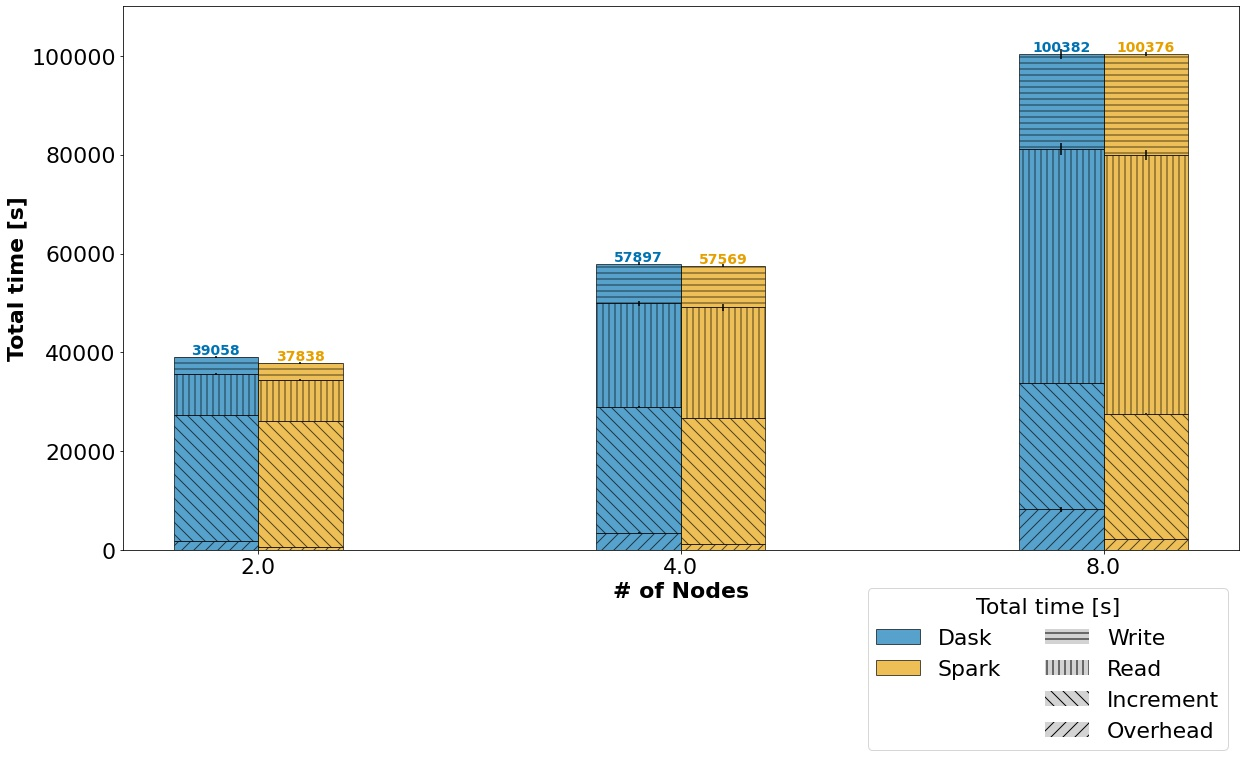
\includegraphics[clip,width=\columnwidth]{figures/stacked_increment_worker.jpg}
	\caption{Increment: varying nodes -- 5000 files, 5 iterations, \SI{1}{\second} delay}
	\label{fig:increment_worker}
\end{figure}
		
Figure \ref{fig:increment_itr} shows the detailed execution time for the \textit{Increment} application while varying the number of iterations.
As expected, the idle time for both engines increases with the number of iterations.
However, idle time for Dask increases significantly faster than Spark, resulting in a \SI{38}{\second} makespan difference for 25 iterations.
		
Figure \ref{fig:increment_itr} also depicts that the total computation time increases as the total I/O time decreases.
This is explained by an I/O bottleneck on the Lustre file system.
When threads are busy with computations, they reduce the contention on Lustre, thus improving I/O speed for individual accesses.
\begin{figure}[!t]
	\centering
	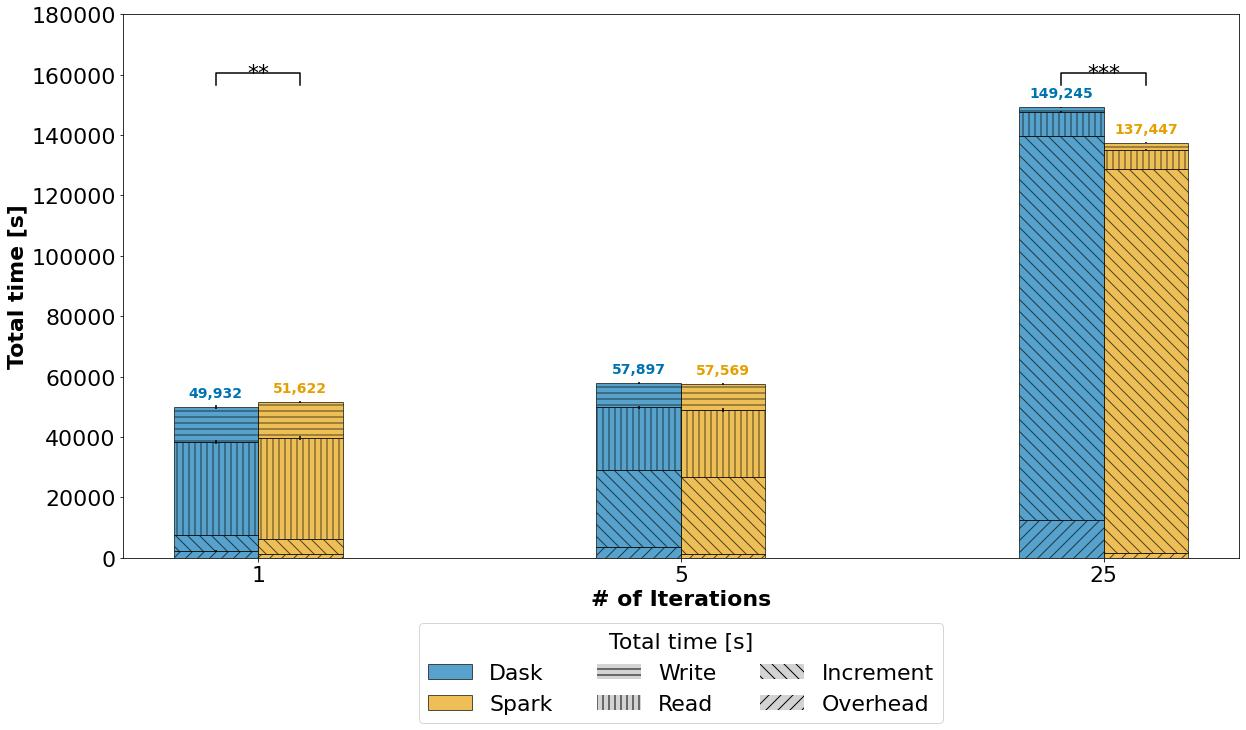
\includegraphics[clip,width=\columnwidth]{figures/stacked_increment_itr.jpg}
	\caption{Increment: varying iterations -- 4 nodes, 5000 files, \SI{1}{\second} delay}
	\label{fig:increment_itr}
\end{figure}
		
Figure \ref{fig:increment_block} shows an increase in \textit{Increment} time.
This is because the application performs an incrementation for each file, thus increasing the computation time.
Similarly to Figure \ref{fig:increment_itr}, increasing the total compute time of the application reduces the total I/O time.
Again, this is explained by the I/O tradeoff between compute time and contention of disk bandwidth.
		
From figure \ref{fig:increment_block} we also observe that Dask has significantly higher idle time than Spark.
However, the total execution time of the application is similar due to the tradeoff between I/O and compute/idle time.
\begin{figure}[!t]
	\centering
	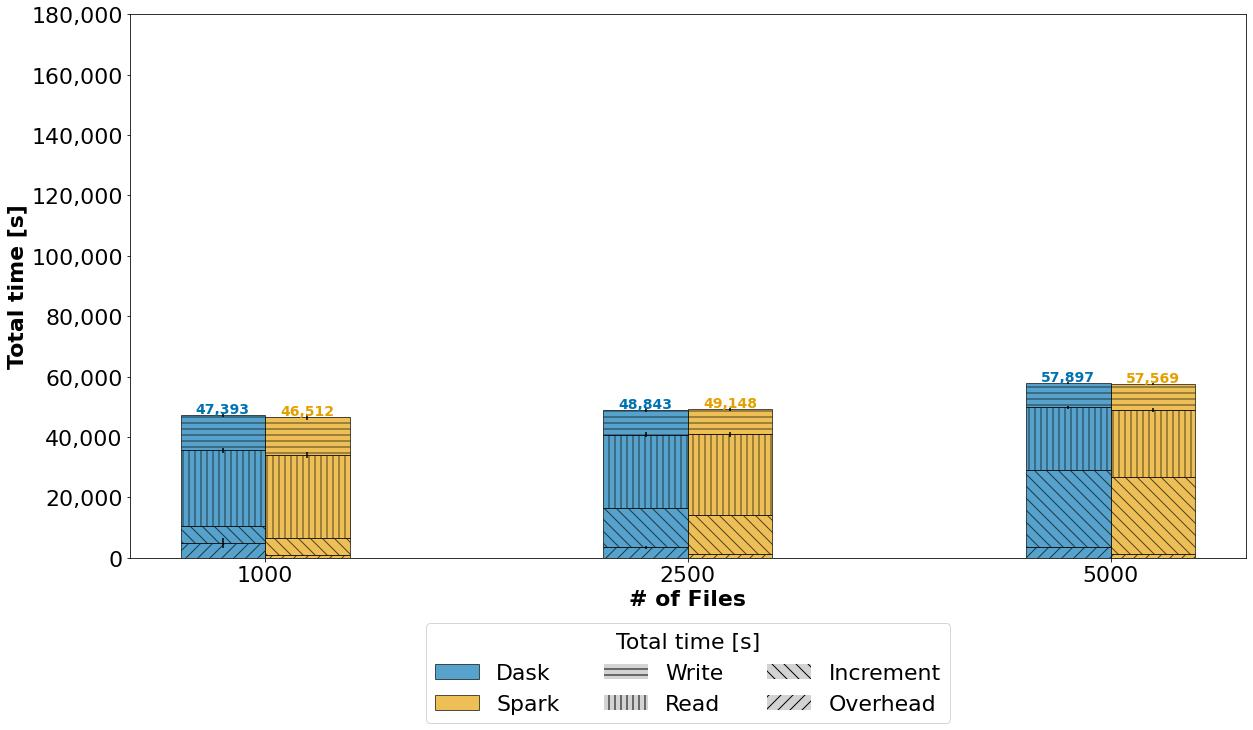
\includegraphics[clip,width=\columnwidth]{figures/stacked_increment_block.jpg}
	\caption{Increment: varying \# of files -- 4 nodes, 5 iterations, \SI{1}{\second} delay}
	\label{fig:increment_block}
\end{figure}
				
\subsection{Histogram}
Figure \ref{fig:histogram_worker} depicts the execution time for the \textit{Histogram} when varying the number of nodes.
Overall, Spark has up to 5\% lower total execution time, with the difference coming from a shorter execution time for \textit{Calculate\_histogram}.
This is unexpected as the code base for both engines is the same, with only the calling APIs differing.
It is most likely due to the use of Dask Bags, which are slower than the other Dask APIs.
As with previous experiments, the overhead for Spark is less and scale better, although compensated by a longer total I/O time.
\begin{figure}[!t]
	\centering
	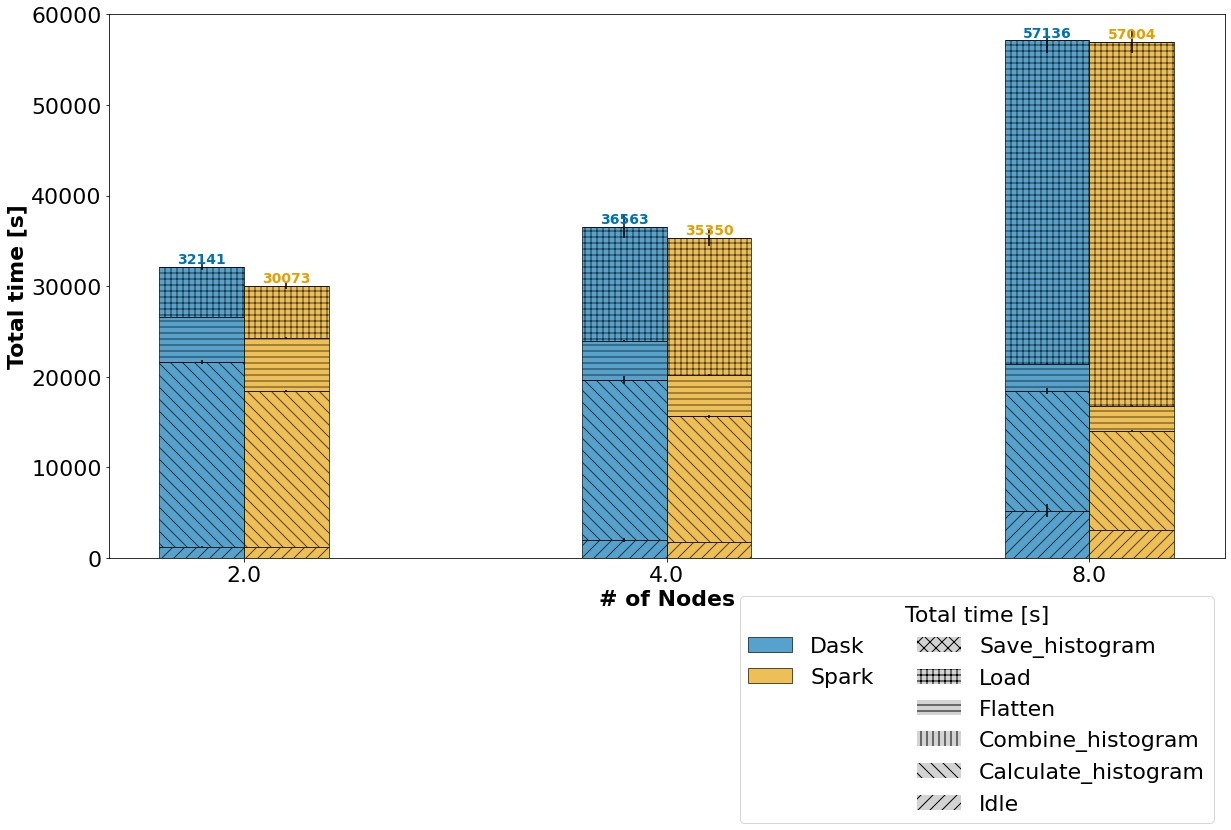
\includegraphics[clip,width=\columnwidth]{figures/stacked_histogram_worker.jpg}
	\caption{Histogram: varying nodes -- 5000 files, 5 iterations, \SI{1}{\second} delay}
	\label{fig:histogram_worker}
\end{figure}
		
Figure \ref{fig:histogram_block} shows the execution time for the \textit{Histogram} when varying the number of files.
The results are similar to varying the number of nodes with Spark having faster compute time for \textit{Calculate\_histogram}.
\begin{figure}[!t]
	\centering
	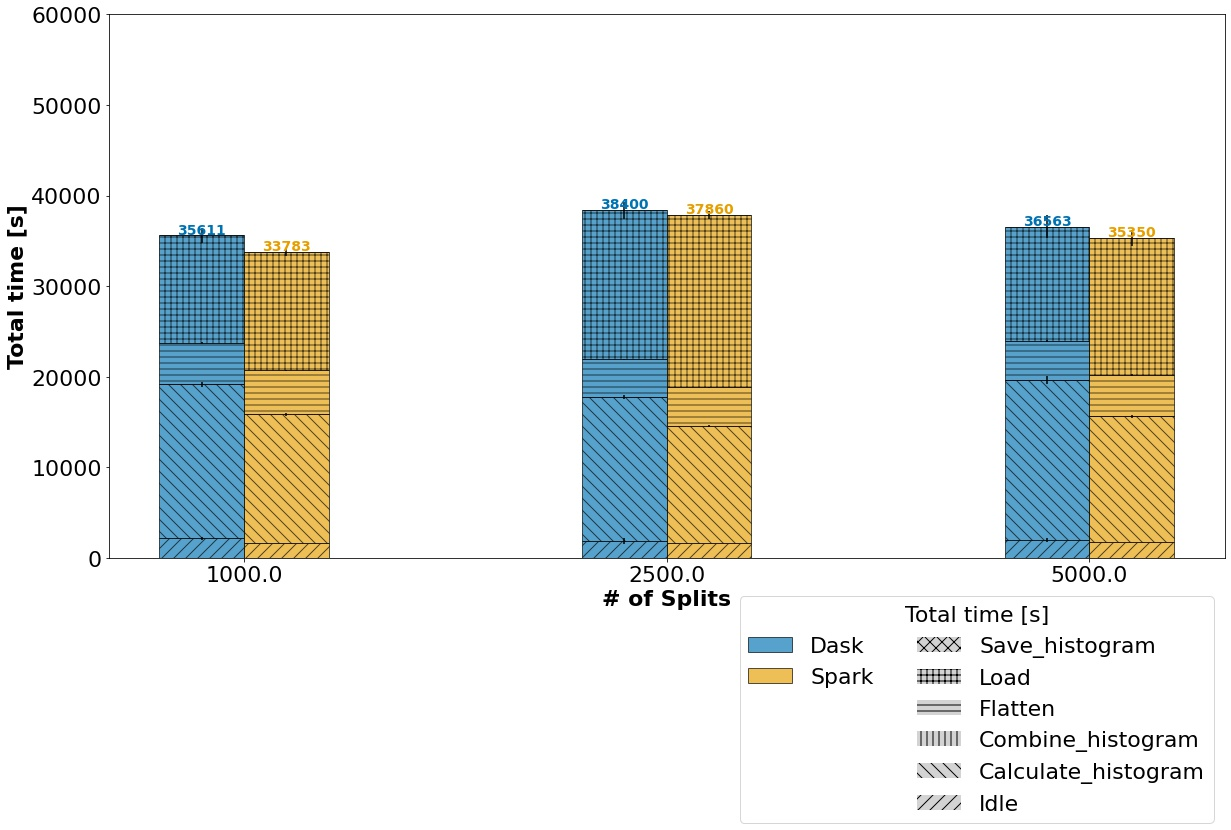
\includegraphics[clip,width=\columnwidth]{figures/stacked_histogram_block.jpg}
	\caption{Histogram: varying \# of files -- 4 nodes, 5 iterations, \SI{1}{\second} delay}
	\label{fig:histogram_block}
\end{figure}

\subsection{Kmeans}
Figure \ref{fig:kmeans_worker} depicts the total execution time for the \textit{Kmeans} application when varying the number of workers.
We observe that Dask is multifold faster than Spark.
Specifically, Spark has much longer idle, \textit{get\_labels} and read time than Dask.
This difference arises from Spark workers restarting due to lack of executor memory, leading to recomputation of tasks.

For Spark, we reduced the number of processes per node from 64 to 32 while keeping the memory the same and found similar execution times.
However, the Spark worker did not restart with a lower process count and no longer recomputed tasks.

We omit the figure when varying the number of iterations as the results are similar to varying the number of workers.
\begin{figure}[!t]
	\centering
	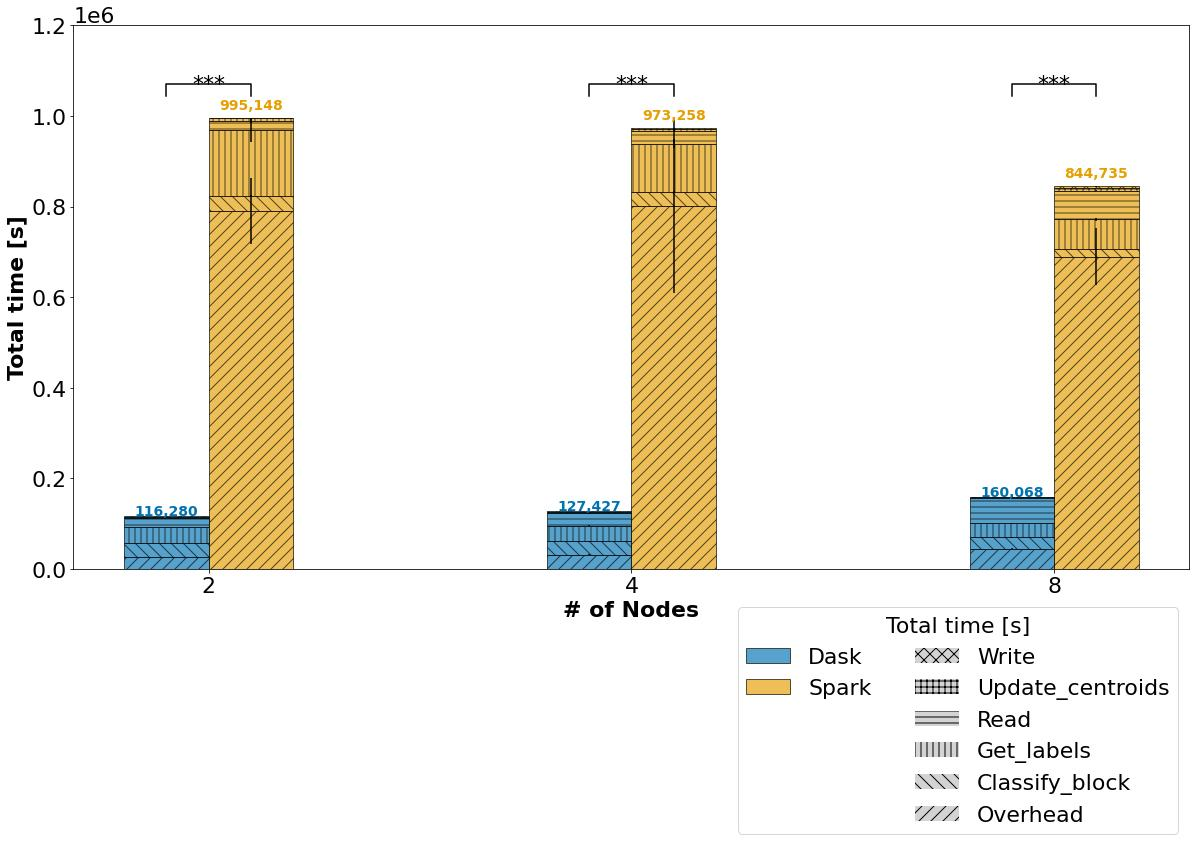
\includegraphics[clip,width=\columnwidth]{figures/stacked_kmeans_worker.jpg}
	\caption{Kmeans: varying nodes -- 5000 files, 3 iterations, \SI{1}{\second} delay}
	\label{fig:kmeans_worker}
\end{figure}

\subsection{BIDS App Example}
Figure \ref{fig:bids} shows the total execution time for the \textit{BIDS App example} application when varying the number of nodes.
We observe that Dask has a significantly lower execution time than Spark, between 10\% to 15\%.
The main difference comes from an increased amount of stagger tasks for Spark, thus increasing the idle time of the application.
Moreover, although minimal, a shorter cluster deployment time for Dask reinforces the difference in idle time.
As with other experiments, the I/O from Lustre affects the scaling of both engines as we increase the number of nodes.
\begin{figure}[!t]
	\centering
	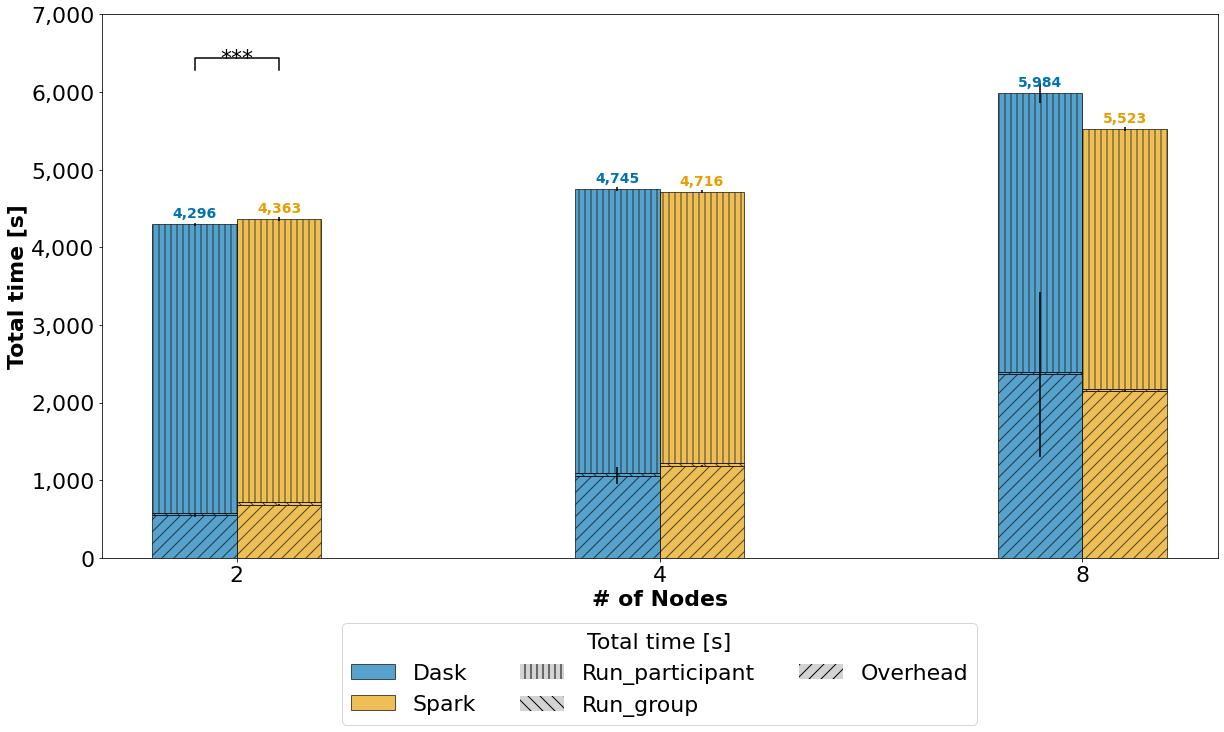
\includegraphics[clip,width=\columnwidth]{figures/stacked_bids.jpg}
	\caption{BIDS App Example: varying nodes}
	\label{fig:bids}
\end{figure}
		
\section{Discussion}
\subsection{I/O bottleneck}
We used Lustre for our share file system as it is a standard solution in HPCs.
The performance of Lustre degrades when a large number of concurrent tasks attempt to perform I/O to the shared file system, as shown in Figures \ref{fig:increment_worker} and \ref{fig:histogram_worker}.
In a previous study \cite{8943502}, we observed nearly no improvement when increasing the number of nodes to process an application while using an NFS.
In this paper, Lustre shows some scaling when increasing the number of nodes, although not linear.
This suggests that increasing the parallelism level of the file system might help alleviate the I/O bottleneck observed.

As in our previous study \cite{8943502}, we observe that the I/O bottleneck from the file system has a lower impact on more compute-intensive applications, such as BIDS App Example.
However, it significantly affects data-intensive applications, such as Increment and Histogram.

These results suggest that increasing the parallelism of the file system is critical when scaling the compute resources to process a data-intensive application.
Otherwise, the compute resource might be underutilized.

\subsection{Tradeoff between overhead and data transfer}
Overall, except for Kmeans, the overhead for Dask is larger than for Spark.
However, the total execution time for both engines is comparable.
This almost exact compensation between the engine overhead and the data transfer time (see for example Figure \ref{fig:increment_worker}) is not surprising.
When there is high contention on the bandwidth of the file system, and in the absence of trashing, desynchronizing the file transfers generally does not reduce the total data transfer time.
To take an extreme example, the makespan of $n$ concurrent file transfer of size $F$ from a file system with a bandwidth $B$ would be $nF/B$,
as the $n$ transfer would share the bandwidth $B$, which is equivalent to sequentially transfer the $n$ files.
i.e., when the bandwidth of the file system is saturated, engine overhead does not increase the makespan as long as it desynchronizes the data transfers.
In a previous study \cite{8943502}, we also observed this tradeoff between overhead and data transfer when the file system was saturated.
It could be interesting to explore strategies that take advantage of this tradeoff to reduce the application makespan.

\subsection{Memory management}
Our Kmeans experiment shows a significant difference between Dask and Spark.
The difference in performance comes from Spark worker restarting due to running out of memory; thus, Spark needs to recompute several tasks
This is unexpected, given that Dask and Spark are configured similarly and use the same amount of resources.
We think those issues arise from a combination of
(1) the reserved memory for the JVM heap space,
(2) the serialization of Python to Java kept in memory,
(3) Spark only using process compared to Dask using threads, thus limiting shared memory,
and (4) different policies to persist data to disk when running out of memory.

When reducing the number of processes from 64 to 32 for Spark (effectively doubling the memory of each process), the total execution time was similar.
However, with only 32, and more memory per worker, Spark no longer recomputed tasks for the Kmeans application.
We suppose that given more memory per thread/process, Dask and Spark would then perform similarly.

\subsection{Comparison to other studies}
Overall, except for Kmeans, our experiments did not show substantial performance differences between Spark and Dask.
In contradiction with the experiments of \cite{Mehta:17}, we found that Dask had a larger overhead than Spark, especially when scaling the number of workers.
However, this was compensated by the overhead and data transfer tradeoff previously.
Since our focus is on data-intensive applications, we conclude that the performance of the engine is equivalent.

The experiments from \cite{Mehta:17} found that Dask has a larger startup overhead than Spark, while another study \cite{8588652} found the opposite.
We did not find significant differences in startup overhead between the engines in this study nor our previous study \cite{8943502}.
Those apparent contractions most likely come from differences in infrastructure and configuration of the engines.

Our results from the Histogram experiments show that the Dask Bags was slower than Spark.
The experiments from \cite{10.1145/3225058.3225128} also found that Dask Bags performed slower than Spark.
We conclude that when using Dask, the other Dask APIs should be favored unless Dask Bags are strictly required.

Our results showed that, for data-intensive applications, increasing the number of workers should only be done if the bandwidth of the file system is not saturated.
Two other studies support this \cite{8943502, 8588652}.
Therefore, it is critical to assure enough bandwidth to the file system before scaling the compute resources for data-intensive applications.
Otherwise, those extras resources might be underused.

\section{Conclusion}
We present a detailed comparison of two Big Data engines, Apache Spark and Dask.
We studied the engines using three synthetic data-intensive applications and a data-intensive neuroimaging pipeline.
Overall, our results showed no substantial difference between the engines.
Although Spark overhead is lower than Dask, Dask performs I/O faster due to a tradeoff between overhead and I/O when the file system is saturated.
For one application, our results showed that Spark used more memory, causing issues with its workers resulting in a significantly faster runtime for Dask.
However, using an infrastructure offering more memory per worker would most likely solve this issue.

These results suggest that future research should focus on strategies to:
\begin{itemize}
	\item Limit the impact of data transfer for data-intensive applications
	\item Reduce the footprint of application memory
	\item Manage the memory of workers more efficiently
\end{itemize}

\section*{Acknowledgment}
% TODO
Mathieu Dugre\'e was funded by an Alexander Graham Bell scholarship from the Natural Sciences and Engineering Research Council of Canada.
\MD{Add other things here..?}


\bibliographystyle{IEEEtran}
\bibliography{IEEEabrv,reference}
\end{document}
